\documentclass{article}
\usepackage{comment}
\usepackage{graphicx}
\usepackage[utf8]{inputenc}
\usepackage[english]{babel}
\usepackage{url}

\begin{document}

\title{Using wavelengths outside of the Telecom spectrum}
\author{Stefan Plug\\Remy de Boer}
\date{\today}
\maketitle

\begin{comment}
\begin{tabular}{|c|c|c|}
\hline 
Version number & Date & Comment \\ 
\hline 
0.1 & 03-01-2013 & Start of of document \\ 
\hline 
\end{tabular} 
\end{comment}

\tableofcontents
\newpage

\section{Preface}
This report is the product of a four week research project done at BeetleFiberOptics, and as part of the Master programme 'System and Network Engineering' at the University of Amsterdam\cite{uva:os3}.

BeetleFiberOptics is part of the Tallgrass company in Amsterdam and is a manufacturer of Coarse Wavelength Division Multiplexing, CWDM. A CDWM is a device which aggregates multiple wavelengths of light onto a single fibre. BeetleFiberOptics would like us to find out if, and how, it could use an extra wavelength outside of the traditional CDWM wavelengths to both monitor an optical fibre and as an extra out-of-band Ethernet network which might be used for network management. Primarily BeetleFiberOptics would like to know if we can use relatively cheap hardware which has the potential of being integrated into their CDWM devices.

We would like to thank the people of BeetleFiberOptics and Tallgrass for their support and knowledge during this project.

\newpage
\section{Summary}
\newpage
\section{Research question}
It is common practice today to use Wavelength Division Multiplexing, WDM, devices on network links to increase the total amount of bandwidth that a single optical network link can carry. The WDM accomplishes this by assigning each input data stream its own unique light wavelength channel, $\lambda$. 
Not every wavelength is suitable for heavy traffic usage because of the physical characteristics of these channels. Our hypothesis is that these channels could be used for lower speed applications such as monitoring and out of band management.
To test our hypothesis we will look at the possibilities of the unused wavelengths outside of the Telecom spectrum.
The main research question will be as follows:
\begin{quote}
\textit{
What applications can the unused wavelengths outside of the Telecom spectrum be used for?
}
\end{quote}

It is important to be able to have an active monitoring system in place which can send out warnings when it detects either degradation of the link over time or a sudden change in the links characteristics, for example when someone places a tap on the link. 

To help us understand how we can effectively monitor an optical link we will ask the following sub-question:
\begin{quote}
\textit{
What optical link characteristics should we monitor?
}
\end{quote}

It could happen that the main traffic interface on a switch shuts down which could potentially shut down that section of the network.
It would be good to have a separate out of band network link up on another interface which could be used to still manage that device.

During this project we will focus on link monitoring and out of band management, but other usages may arise during our research.
If this should happen we shall try to document them.

\newpage
\section{Telecom spectrum}
When we look at the wavelengths used for telecommunication we can see that the ITU-T has defined the following bands as shown in table \ref{tab:bands}
\begin{table}[h]
\centering
\begin{tabular}{|c|c|c|c|}
\hline 
\textbf{Band} & \textbf{Descriptor} & \textbf{Range [nm]}\\ 
\hline 
O-band & Original & 1260 to 1360 \\ 
\hline 
E-band & Extended & 1360 to 1460 \\ 
\hline 
S-band & Short wavelength & 1460 to 1530 \\ 
\hline 
C-band & Conventional & 1530 to 1565 \\ 
\hline 
L-band & Long wavelength & 1565 to 1625 \\ 
\hline 
U-band & Ultra-long wavelength & 1625 to 1675 \\ 
\hline 
\end{tabular} 
\caption{ITU-T Bands\cite[p. 134]{itu-t:manual2009}
\label{tab:bands}
}
\end{table}

The ITU-T further describes the U-band as:
\begin{quote}
In some cases it is desirable to perform a number of maintenance functions (preventive, after
installation, before service and post-fault) on fibre cables in the outside plant. These involve
surveillance, testing, and control activities utilizing optical time domain reflectometer (OTDR)
testing, fibre identification, loss testing, and power monitoring. A wavelength region, that is
intended to be never occupied by transmission channels, may be attractive for maintenance,
even if enhanced loss occurs. The U-band has been defined exclusively for possible
maintenance purposes.
\end{quote}

The ITU-T's intended use of the U-band corresponds with our own objectives, it is therefore obvious to us that we will further concentrate on this band.

\subsection{Choosing a wavelength}
The U-Band reaches from 1625nm to 1675nm. When choosing a wavelength we need to make sure that we have the least amount of energy loss or attenuation when transmitting light.
The amount of attenuation depends both on the fibre type and wavelength which is used. 

The main reason of our research is to look at potential uses of the unused channels at the edge of the L-band in a WDM system.
Because of this we can safely assume that the fibre optical cable used is a single mode fibre which supports C+L band WDM systems.
If the link was not used in a WDM set up, then there would be no reason to use the unconventional U-band.

The ITU-T has several standards ranging from G.652 to G.656 which specify single mode optical fibres\cite[chap. 6-7]{itu-t:manual2009}, of which none have official support for the U-band.
The U-band channel we choose should for this reason be as close to the L-band as possible to keep the wavelength closer to the cable's specifications.

Figure~\ref{fig:attenuation} on page~\pageref{fig:attenuation} shows attenuation as a function of the wavelength of an unbent fibre. We can see that in the case of the U-band there is a gradual upward slope as the wavelength increases.
\begin{figure}[h]
\centerline{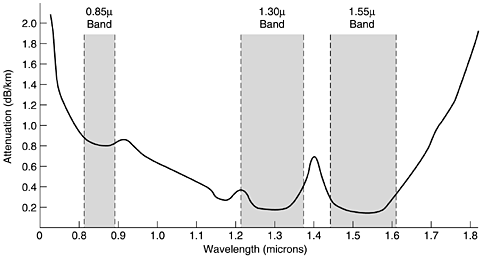
\includegraphics[scale=0.5, trim = 0mm 0mm 0mm 0mm]{images/attenuation.png}}
\caption{Attenuation of light through fibre in the infra-red region.\cite[fig 2-6]{tannenbaum:networks}}
\label{fig:attenuation}
\end{figure}

Figure~\ref{fig:attenuation-bends} on page~\pageref{fig:attenuation-bends} shows the effect of fibre bends on attenuation. Here we can see again that it is better to choose a wavelength as close to the L-band as possible.
\begin{figure}[h]
\centerline{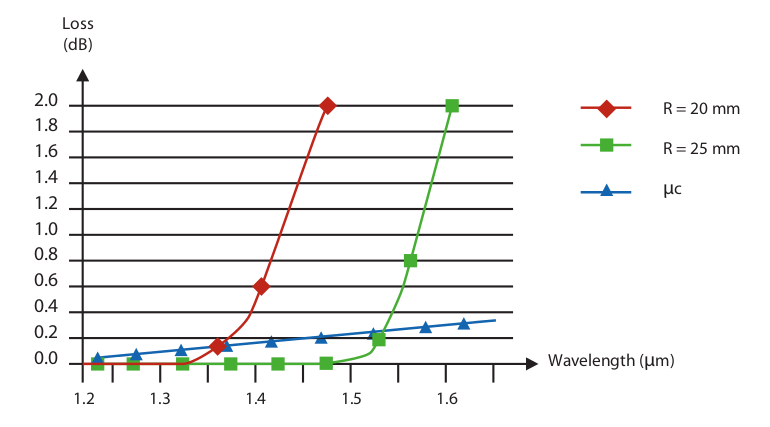
\includegraphics[scale=0.3, trim = 0mm 0mm 0mm 0mm]{images/attenuation-bends.png}}
\caption{Effect of fibre bends on attenuation.\cite[p. 27]{refguide:2011}}
\label{fig:attenuation-bends}
\end{figure}

Because the U-band begins with 1625nm we think that this would be the best wavelength to use.

\newpage
\section{Proof of Concept}
To test our hypotheses we were initially provided with two Inteno XG6746\cite{Inteno:XG6746} switches and four 1625nm SFP optics by BeetleFiberOptics.
It is in the interest of BeetleFiberOptics that we use this relatively cheap equipment instead of specialised, and usually more expensive fibre monitoring equipment.
The Inteno XG6746 switches have one modular SFP fibre optic port in which we can place the optics to be tested. 

We would like the fibre optic switches to communicate with each other so they can exchange statistics about their fibre optics and use these statistics to create MRTG\cite{MRTG:MRTG} graphs that could show interesting trends which might be an indicator of fibre degradation over time.

\subsection{Inteno XG6746}
The Inteno XG6746 runs on the software image \texttt{XG6746\_4.02ITT24.01\_20121022}.
Because of the closed nature of the software we were not able to directly install programs or scripts which we needed to generate traffic on the fibre link directly.
Before the start of our research project we had been informed that customizable software would be made available for these switches so we could write our own testing modules.
This, however, never happened and as such we had to come up with another solution.

We tried to install several open-source operating systems on the switches, unfortunately none of them would work. To still be able to run diagnostic tests we decided to attach a Raspberry Pi to to the switch via Ethernet which can both generate traffic and do periodic polling via SNMP.
Ideally all the functions performed by the Raspberry Pi would be integrated into the Inteno XG6746, however to simplify matters we chose to use a Raspberry Pi as it boasts a full-fledged Linux environment, Raspbian\cite{raspbian:raspbian}.

The Inteno XG6746 allows us to read out the following information about the optic:
\begin{itemize}
	\item Vendor Name : EOPTOLINK INC   
	\item Vendor OUI  : 00 00 00
	\item Vendor PN   : EOLS-1603-29SD  
	\item Vendor rev  : 1.0 
	\item Temperature : 62.559 C
	\item Voltage     : 3.19 Volts
	\item Bias        : 8 mA
	\item Tx Power    : -5.65 dBm \emph{probably wrong}
	\item Rx Power    : -0.03 dBm \emph{probably wrong}
\end{itemize}

As seen above we can read out the optics’s Rx and Tx, however, we do not know in what format these values are presented. An example of the readout is shown in table \ref{tab:crazy-inteno} on page \pageref{tab:crazy-inteno} in which we show the represented values of two connected Inteno XG6746 switches using 1550nm optics with a 25KM fibre and where we compare the Rx value with that of a separate Optical Power Meter, a Fujikura FID-25R.

\begin{table}[h]
\centering
\begin{tabular}{|c|c|c|c|}
\hline 
\textbf{Switch} & \textbf{Tx} & \textbf{Rx} & \textbf{OPM measured Rx}\\ 
\hline 
Sw1 & -4.61 dBm & -0.44 dBm & -9.8 dBm\\ 
\hline 
Sw2 & -4.86 dBm & -0.83 dBm  & -12.4 dBm \\ 
\hline 
\end{tabular} 
\caption{Tx and Rx values of two connected Inteno XG6746 switches}
\label{tab:crazy-inteno}
\end{table}

The web-based GUI shows us that the values should be in dBm, but this makes no sense as the Tx is always lower then the Rx, this would indicate an increase of power in transit. This effect also increases when we introduce an attenuator on the link. Even if we would assume that this is the result of a simple mix-up of Rx and Tx then these values still make no sense because we get totally different values when measuring the actual output with the optical power meter. Also when we assume that these values are in fact measured in milliwatts then these values still make no sense as the values are negative. When the optics are placed in a different type of switch then we do get expected values which would indicate that this problem does not lie in the optics, but rather in the switch itself. We expect this to be a software bug which can be resolved in the future. For this reason we have decided to still use the Inteno XG6746 for testing out-of-band management. For correct fibre attenuation monitoring we had to use another type of switch, a Zyxel XGS4728F.

Although the Zyxel XGS4728F does show us the correct Tx and Rx values for the 1625nm optics, it does not allow them to actually come up. The reason for this is that the optics are only 100-mbit which the Zyxel XGS4728F does not support. 

We can calculate how much dB attenuation is present on the fibre between two switches by subtracting the Tx dBm on switch1 with the Rx dBm on switch2, $dB=Tx_1-Rx_2$. We think it would also be interesting to keep track of the temperature of the Tx optic because this might influence the precise Tx wavelength, and thus attenuation.

Our particular hardware situation requires us to build two different networks. Our primary test network will proof that an Ethernet network using 1625nm optics is possible, and our Attenuation network will prove that we can monitor the attenuation of a fibre link over time.

\subsection{Primary test network}
\begin{figure}[h]
\centerline{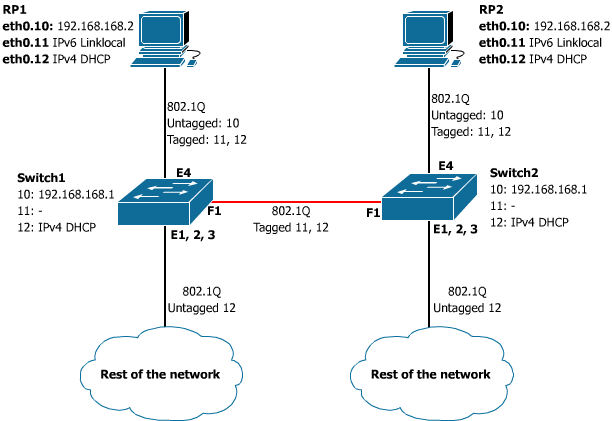
\includegraphics[scale=0.4]{images/PoC_all.png}}
\caption{Network diagram of the out-of-band management network}
\label{fig:poc_all}
\end{figure}

Figure~\ref{fig:poc_all} on page~\pageref{fig:poc_all} shows our primary test network which uses the Inteno XG6746 switches. A secondary goal of this network was to make it as 'plug-and-play' as possible, meaning that an engineer shouldn't be required to do much configuring. This network should proof that we can use the 1625nm wavelength to create a Ethernet link which can be used alongside the regular wavelengths. The RP devices will automatically use SNMP to poll Rx and Tx data from their nearest switch, and send the Rx data to the other RP device for comparison. It is important to note that we use 3 separate VLANs for this. 

The purpose of \texttt{VLAN-10} is to create a single unit out of 1 Raspberry Pi and 1 monitored switch. This way \texttt{RP1} will only monitor \texttt{Switch1} although \texttt{Switch2} uses the same default IPv4 address as \texttt{Switch1}. In the ideal situation where the \texttt{RP\#} and \texttt{Switch\#} would be combined into 1 device this VLAN would be obsolete.

\texttt{VLAN-11} is used to exchange data between 2 \texttt{RP\#} devices. This VLAN creates a group of 2 \texttt{VLAN-10} units using the fiber optics in port \texttt{F1} on \texttt{Switch\#}. The \texttt{RP\#} devices use an IPv6 Link local address, this is done so there is no need to manually configure an IP address when 2 \texttt{VLAN-10} units are connected to each other. The 2 RPs can discover each other by sending a ping to IPv6 multicast address \texttt{FF02::1} to which all IPv6 linklocal hosts should listen and reply too\cite{ietf:rfc4291}. After the RP knows the IPv6 address of a potential neighbour it will do a simple check to see if that neighbour is indeed our polling partner and not some rouge computer. It will do this by sending a SHA256 hash of a common pre-shared password plus its own linklocal IPv6 address which should protect against a simple re-play attack.

\texttt{VLAN-12} is used to connect our devices to the rest of the network and thus might be used for out-of-band management.


\subsection{Attenuation test network}

\begin{figure}[h]
\centerline{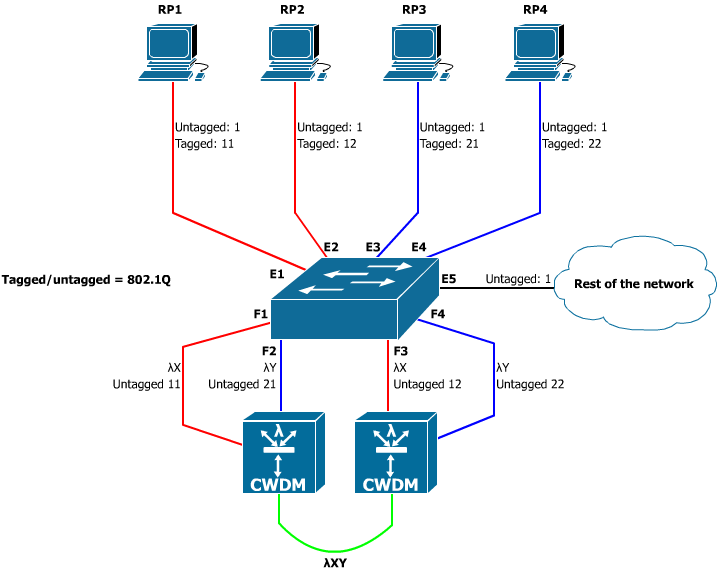
\includegraphics[scale=0.4, trim = 0mm 0mm 0mm 0mm]{images/CWDM.png}}
\caption{Network diagram of the attenuation test network}
\label{fig:CWDM}
\end{figure}

Because of the dBm representation problem of the Inteno XG6746 switches we had to do create a alternate network using another switch type which does display the Tx and Rx values correctly. The Zyxel XGS4728F does display the correct values, but there was only one available to us, therefore a new network set-up was needed. The Attenuation test network diagram is shown in figure \ref{fig:CWDM} on page \pageref{fig:CWDM}.

The Zyxel XGS4728F switch does have one major flaw, it does not support 100-mbit speed optics to come up, which our 1625nm optics are. Luckily it does still give the correct Tx and Rx values for these optics when they are connected to each other with a fibre.

We can both test our dBm exchange script and poll from the 1625nm optics because we can let the RPs poll not only from the optics in their own VLAN, but also from the 1625nm optics.

\newpage
\section{Tests}
We would like to find out if we can use the 1625nm wavelength to do reliable tests of a fibre. First we will establish a base test using a well-known wavelength used for optical networking. After the base-test we will compare this to the 1625nm wavelength.

Before we will use our test-network we will test this with the reliable Bit Error Rate testers so we also have a base to compare our own set-up with.

The set of tests will consist of the following three parts:
\begin{itemize}
\item Measuring the difference between Tx and Rx values at either end of the fibre link.
	\begin{itemize}
	\item This test will be performed on the same fibre using three different sets of optics operating of different wavelengths.  We will use two common wavelengths as a base reading to compare to the results of the 1625nm wavelength.
	\end{itemize}
\item Sending a steady stream of UDP packets across the fibre at 10Mb/s.
	\begin{itemize}
	\item This will show if packets are being lost while travelling across the fibre. Our preliminary tests have shown that excessively bending a fibre will result in severe packet loss.
	\end{itemize}
\item Running traditional OTDR tests across the fibre
\end{itemize}

The first two of these tests will be done using our test set-up.
Especially for the first test it is important to bear in mind that we are getting our Tx and Rx values from the digital diagnostic information provided by the optic.
This information has an error margin which can be vendor specific, but may be at most 3dBm, as stated in the SFF-8472 Specification for
Diagnostic Monitoring Interface for Optical Transceivers\cite{SFF:DDM}

\subsection{bla}
For our main tests we have used 1625nm optics.
To compare we also ran the same tests on 1550nm and 1610nm optics.
To validate our test-network itself we will also run similar tests on more specialised equipment using the same optics.
In theory these optics should return the same values, regardless of which equipment they are plugged into.
The optics return their values through the standardised digital diagnostics monitoring interface using i$^2$c, this standard defines which values are measured and how the information is stored.\cite{SFF:DDM}
In practice, we have noticed that equipment manufacturers sometimes seem to change these values before displaying them.
A prime example are the Inteno switches used as the core of our tests.
The Rx and Tx values returned by these switches deviated from the actual values so much that it was impossible for us to spot any clear relation between the presented values and the values as measured by a separate optical power meter.
After some investigation our tests showed that the values presented by the Inteno switches do bear resemblance to the actual values, however they are modified in such a way as to make them completely useless.
For example: the value for Rx power actually was higher than the measured Tx value, and would even increase when the signal was purposefully attenuated.

As our initial set-up seemed unreliable for power measurements, we built another.  This time we used a 28 port ZyXEL switch to which we connected all our devices and fibres.
Using VLANs we set up connections between two Raspberry Pi's via a 25 kilometre fibre cable.
This 25 kilometre cable could then be used to test the attenuation of each signal wavelength over a reasonably long distance.

\subsection{Testing equipment}

PUT ALL HARDWARE WE USED IN THIS CHAPTER INCLUDING ALL OPTICS AND OTDRs
\begin{itemize}
\item Inteno XG6746 \cite{Inteno:XG6746}
\begin{itemize}
\item Broadcom 6338
\item Marvell 88E6161
\item 8 MB Flash
\item 32 MB RAM
\end{itemize}

\item Raspberry Pi - Model B

\item Optics:
\begin{itemize}
\item SFP
\item EOptolink
\item EOLS-1603-29SD
\item 1625nm
\end{itemize}
\end{itemize}

%\subsection{Results}
%After running the tests it quickly became apparent that the 1625nm band is very susceptible to attenuation.

\subsection{Rx- Tx values}
We started off by using Bit Error Rate Testers (BERT) to read the attenuation of the light signals across different wavelengths and cable lengths.
The following wavelengths were tested:
\begin{itemize}
	\item 1550 nm
	\item 1610 nm
	\item 1625 nm
\end{itemize}

For each of these wavelengths we tested four different optics, to make sure we had somewhat reliable results to accurately portray the attenuation of each wavelength.
All of the used optics were also designed for use over a range of 40 kilometres.
Each of these optics was then run across a one metre and a 25 kilometre fibre cable.
These tests were then also performed using a different Bit Error Rate Tester, 
This results in the following tables, showing the average attenuation for each wavelength and fibre cable length:

\begin{table}[h]
\centering
\label{tab:attenuation-table-ber}
\begin{tabular}{|c|r|r|}
\hline 
\textbf{Wavelength} & \textbf{1 M} & \textbf{25KM}\\ 
\hline 
1550nm & -0.05 dB & 8.3625 dB\\ 
\hline 
1610nm & 0.0875 dB & 7.975 dB\\ 
\hline 
1625nm & 2.275 dB & 14.325 dB\\
\hline
\end{tabular} 
\caption{Wavelength attenuation as measured with BERT}
\end{table}

\begin{table}[h]
\centering
\label{tab:attenuation-table-ofr}
\begin{tabular}{|c|r|r|}
\hline 
\textbf{Wavelength} & \textbf{1 M} & \textbf{25KM}\\ 
\hline 
1550nm & 0.4425 dB & 9.2325 dB\\ 
\hline 
1610nm & 0.62375 dB & 9.2825 dB\\ 
\hline 
1625nm & 2.25125 dB & 14.95625 dB\\
\hline
\end{tabular}
\caption{Wavelength attenuation as measured with BERT \& OFR}
\end{table}

As you can see, the 3 dBm error margin for the digital diagnostics monitoring distorts the results of the BERT measurements using the one metre cable quite significantly.
For these tests the attenuation measured with the OFR seems more reliable, however only the Rx is measured by the OFR.
The Tx is still provided by the DDM interface and may have a larger deviation.

Regardless of this deviation, it is clear that the 1625nm wavelength suffers from considerably more attenuation than the other tested wavelengths.
The 1625nm optics are designed to handle at most 30dB difference between Tx and Rx power, so this test across 25 KM still falls well within the defined range of the optics.
The downside to the 1625nm wavelength suffering from such increased attenuation is that more power will be needed to cover larger distances, compared to regular C- and L-band wavelengths. 

\subsection{Ethernet link reliability}
After establishing that the 1625nm optics seemed to communicate properly, we set up an Ethernet link using two Inteno switches.



\section{Ethernet using 1625nm}
Up until now the 1625nm band has been used for monitoring, however so far it has been mainly used for out-of-band OTDR testing.
Especially in DWDM systems the 1625nm band is used for these OTDR tests to tell if the monitored fibre is still in good condition to support wavelengths in the L- and U bands.
What has surprised us somewhat is that 1625nm optics are not readily available, meaning the wavelength is not regularly used for data communications using Ethernet.
The tests we have performed during our research have shown the 1625nm band to be a lot more sensitive to attenuate through bending, temperature differences and distance.
Regardless of these drawbacks, the 1625nm wavelength has proven to allow for the creation of stable Ethernet links.




\newpage
\section{Conclusion}
\bibliographystyle{plain}
\bibliography{bibliography}

\end{document}
